\documentclass{ximera}

\title{This is the sample!}
\author{JIM!}

\begin{document}
\begin{abstract}
Testing interactives and ff.
\end{abstract}
\maketitle

waffle and Jeff and fine.

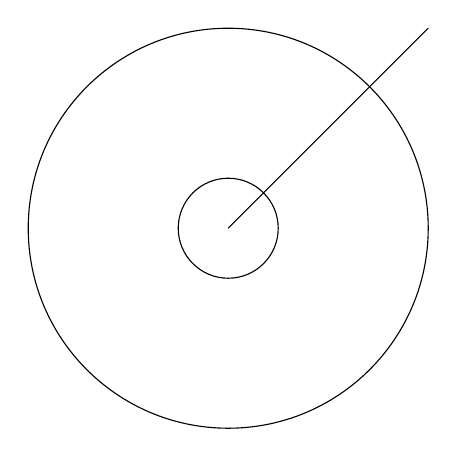
\begin{tikzpicture}
  \draw (0,0) circle (1in);
  \draw (0,0) circle (0.25in);
  \draw (0,0) -- (1in,1in);
\end{tikzpicture}

\begin{problem}
  \begin{multipleChoice}
    \choice{Hello}
    \choice{What?}
    \choice{Goodbye}
  \end{multipleChoice}

  \begin{multipleChoice}[id=mc]
    \choice[value=hello]{Hello}
    \choice[value=what,correct]{What?}
    \choice[value=goodbye]{Goodbye}
  \end{multipleChoice}

  You picked \js{mc}.

  \begin{multipleChoice}
    \choice[correct]{Right}
    \choice{Wrong}
  \end{multipleChoice}

  \begin{multipleChoice}[id=tf]
    \choice[correct,value=t]{T}
    \choice[value=f]{F}
  \end{multipleChoice}
\end{problem}

\begin{problem}
  Find two integers which sum to twenty five.

  % this should be a callback potentially (I guess if it returns a function?)
  \begin{validator}[a+b==25]
    $\answer[format=integer,id=a]{16} + \answer[format=integer,id=b]{9} = 25$.
  \end{validator}
\end{problem}

\begin{problem}
  String equality is like $\mbox{Dog} = \answer[format=string,id=word]{Dog}$.  Or just $\answer[format=string]{WHEE}$.

  So the format determines a default validator, like format=string determines validator=stringEquality.  And now I removed the CDATA.
\end{problem}

\begin{problem}
  The tolerance (0.01) means $8 \approx \answer[tolerance=0.01,id=x,format=integer]{8}$
  
  \begin{feedback}
    The answer is definitely more than five.
  \end{feedback}

  \begin{feedback}[x==10]
    The answer is certainly not ten.
  \end{feedback}
\end{problem}

\begin{javascript}
  letters = word.length;
\end{javascript}

And another one.  $x + 10 = \js{x+10}$ is equal to \js{x + 10}.

And the word ``\js{word}'' is \js{letters} letters long.

$\js{2+5} = 7$.

\end{document}
